% Subsection 3.2: mwi

\subsection{Middleware Interface}
\label{MWI}

For DC2, we split the LSST framework into two parts: the middleware
interface, or MWI, and the application framework, or FW (\Sec{FW}).
Each lies in its own namespace (\code{lsst::mwi} and \code{lsst::fw}).

The middleware interface provides general-purpose services to the
application framework and the distributed processing pipeline framework.
It serves to isolate the application from the details of the underlying
infrastructure.  Among these services are memory leak checking and
debugging, exception reporting with the capability to attach flexible
data describing the problem, a general metadata class, a factory for
LSST objects, a class allowing text-file-based configuration of all
application components, and a framework for flexibly handling
persistence and retrieval of application objects.  In addition, a
database schema for storing DC2 application data, metadata, and
provenance information was developed.  In DC2, MySQL was used to
implement this schema, but another RDBMS could have easily been
substituted.


\subsubsection{The Citizen Class}

\paragraph{Description and Usage}

\code{Citizen} is a C++ class designed to support memory leak checking and
debugging.  Most DC2 C++ classes are subclasses of \code{Citizen}, whose name
was chosen to indicate that it encapsulates the minimum interface
required of well-behaved LSST classes.  All instances of such classes
are registered in a table, and their allocation and deallocation is
tracked.  A static method allows the table to be dumped, ensuring that
no unexpected instances are left at the conclusion of an execution.
Additional methods make it easier to set breakpoints on allocation or
deallocation of instances.

\code{Citizen}'s memory leak checking capability was used throughout the unit
test suites and in debugging the pipeline framework, although the
extensive use of \code{boost::shared\_ptr} throughout the C++ code
helped to minimize memory leaks and thus the need for \code{Citizen}-level
debugging.

Another feature of \code{Citizen} is the unique identifier associated with each
instance upon registration at allocation time.  This identifier provides
a valuable debugging tool.  For example, we can note that a particular
\code{DiaSourceVector} has identifier 19580205 and can ask to set a
breakpoint when that object is constructed or otherwise manipulated;
furthermore, these identifiers are preserved across a recompilation,
provided that the order of allocation of instances does not change.

\paragraph{Issues and Lessons Learned}

Some data instances are allocated and initialized statically, either at
program startup or at shared library load time.  Most such items are intentionally
never deallocated.  If these items are \code{Citizen}s, they appear as memory
leaks.  Some such items were made non-\code{Citizen}s; for others that might
usefully employ \code{Citizen}'s other capabilities, a \code{markPersistent()}
method was added that allows them to be tracked but ignored for leak
checking.

\code{Citizen} uses a constructor that takes a \code{std::type\_info} reference
to enable it to keep track of the types of instances registered with it.
For direct subclasses of \code{Citizen}, it is simple to have all constructors
initialize \code{Citizen} with the type information.  If these classes are ever
to be subclassed, however, they must define appropriate constructors
taking \code{std::type\_info} arguments in order to capture the subclass
type information.

\subsubsection{The DataProperty Class}
\label{DataProperty}

\paragraph{Description and Usage}

\code{DataProperty} is a general-purpose class that can represent a
hierarchical set of key/value pairs.  In fact, it is slightly more
complex: each \code{DataProperty} is either a key/value pair itself or a key
with an attached, subordinate ordered list of key/value pairs.  Such a
list may include duplicate keys.  Keys in a \code{DataProperty} are always
strings, and values may be of any C++ type.

\code{DataProperty} is used wherever generic mutable key/value metadata
is desirable, including:
\begin{itemize}
\item FITS headers associated with an image,
\item Data associated with a pipeline event,
\item Data associated with an exception, and
\item Parameters that help determine to where data is to be persisted
or from where it is to be retrieved.
\end{itemize}

The original \code{DataProperty} design in \Fig{dataproperty-design}
included the classes \code{AttributeDefinition} and \code{AttributeDictionary} 
to describe the allowable keys, value types, and potentially even value
ranges for \code{DataProperties}.  These facilities were not implemented for
DC2.

\begin{figure}[htbp]
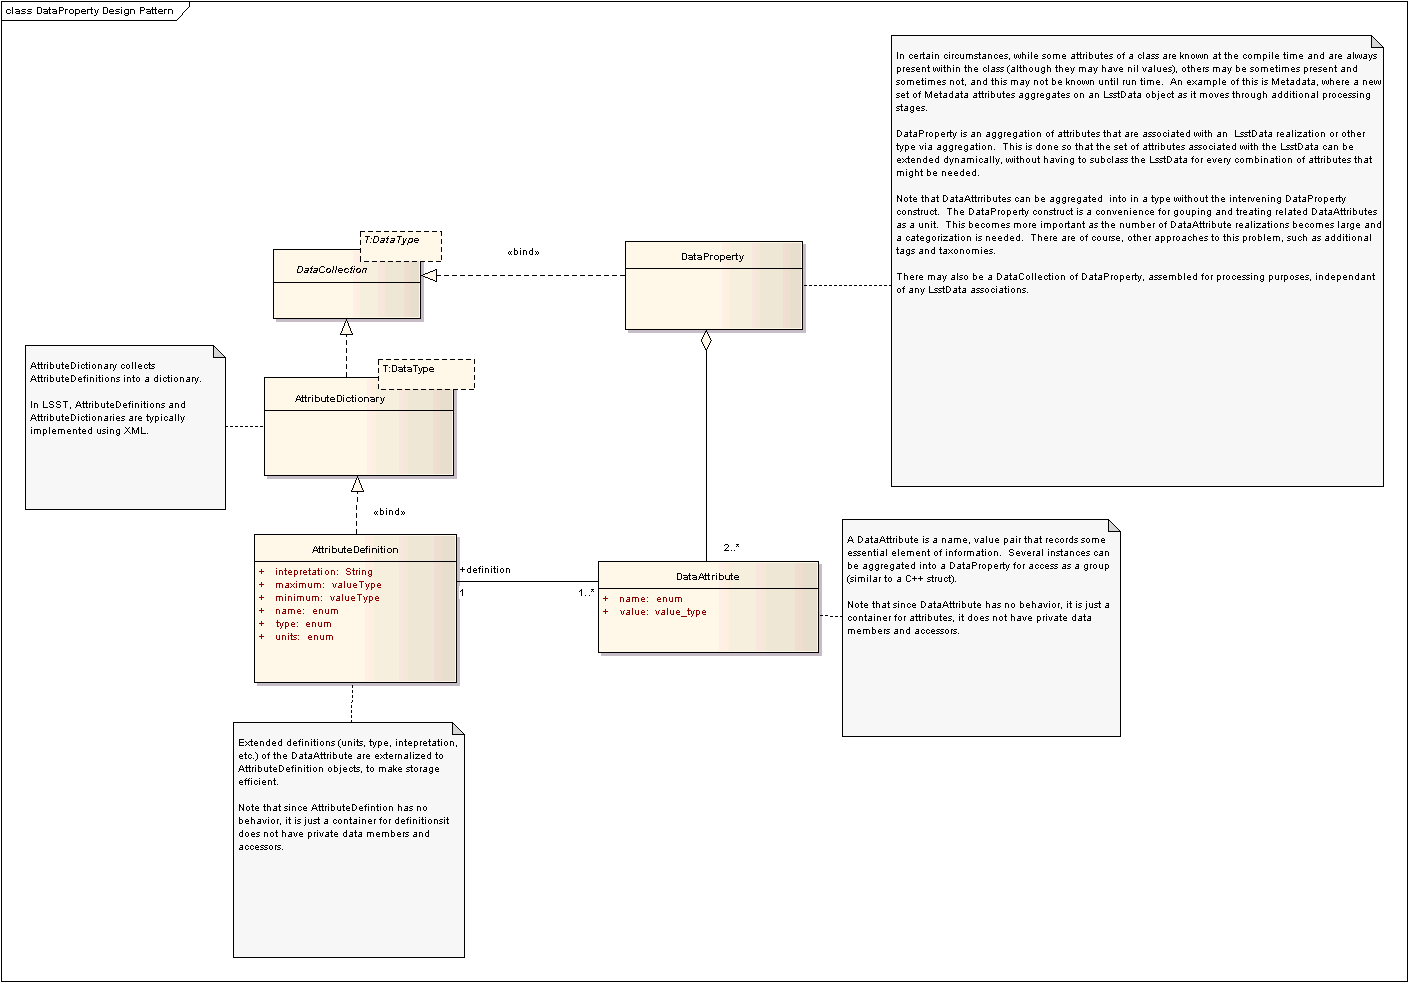
\includegraphics[width=\textwidth]{figures/DataPropertyDesign.png}
\caption{\code{DataProperty} Design Pattern}
\label{dataproperty-design}
\end{figure}


\paragraph{Issues and Lessons Learned}

The biggest issue with DC2's version of \code{DataProperty} is its data model,
which conforms best to FITS headers in allowing duplicate keys and being
order-sensitive.  Neither of these capabilities is characteristic of
the familiar key/value dictionary 
used by \code{std::map}, \code{std::hash\_map}, Java and Python
dictionaries, and the LSST \code{Policy} class (\Sec{Policy}). 
Ordered lists with duplicate keys can still be represented 
in a dictionary by using a single key
having an ordered list of values, however, and we will investigate reconciling the
data models of \code{DataProperty} and \code{Policy} in DC3.

Another issue that arose with \code{DataProperty} stemmed from its
implementation in terms of \code{boost::any}.  While this allowed any
C++ object to be inserted as a value --- a highly desirable feature --- it
meant that the recipient of a \code{DataProperty} needed to know the type of
value associated with each key at compile time before extracting that
value.  Even having execution-time metadata (e.g. from a \code{Definition}
class) describing the value type
associated with each key would not resolve this problem, as a type
switch would still be necessary.  While having such type information at
compile time (or code writing time) allows C++ to select the appropriate
value-extracting method, such code is particularly unnatural in Python,
where types are assumed to be dynamic.  In addition, explicit
construction functions for \code{DataProperties} had to be defined for Python
since some C++ types, such as \code{float} or \code{int64\_t}, are
inaccessible via implicit type matching in SWIG.  Adding utility
functions to extract integral types (regardless of size), real types, or
string types may help.

The initial \code{DataProperty} design had no easy way to combine two \code{DataProperty}
nodes.  We added an \code{addChildren()} method to allow all of the
children of one node to be added to another, replacing any of the same
name if already present.

\code{DataProperty} provides a powerful generic mechanism for sharing and
transmitting data, potentially finding uses even for communicating data
between functions in C++ or Python.  Programmers will need to be careful
to use this capability only when required, however, as passing function
arguments as a \code{DataProperty} instead of as explicit arguments may reduce
the type-safety, documentability, and debuggability of the code.

\subsubsection{Exception Classes}

An \code{ExceptionStack} class was defined to act as the main LSST exception
type.  Implementing this as a stack allows exception handlers to rethrow
exceptions without losing any underlying information.  All LSST
exceptions are subclasses of \code{ExceptionStack}.

Each exception (or level of the exception stack) can also contain a
\code{DataProperty} so that machine-interpretable key/value pairs can be
attached to the exception.  These key/value pairs are in addition to
the exception type and a human-readable exception message.

In DC2, exceptions were sometimes caught by calling code based on their
type information alone; if not, they propagated to the pipeline
framework, which handled them in an intelligent but generic,
type-independent and data-independent, fashion.  In DC3 and subsequent
Data Challenges, application-level exception handling is expected to
become more prevalent, making use of the stack and attached data
functionality described above.


\subsubsection{Trace and Logging Classes}

\paragraph{Description and Usage}

Two similar facilities were developed for emitting messages for
display that indicate what is happening in the code as it executes.
The Trace facility was developed first to serve the immediate
needs of the development phase as a debugging tool.  Later, a more
sophisticated logging facility was developed to support use cases
beyond simple debugging.  Building on the Trace design (as well as
some of the same underlying code), the logging system allows messages
to be automatically timestamped and collected from the many parallel
processes in an effective way.

The Trace facility is made up primarily of a \code{Trace} class
and a \code{TTrace} template that enable developers to produce debugging 
messages; these messages may be left in the source code
and selectively enabled by the user.  Both classes associate the
messages with a component name, which is defined hierarchically, and a
verbosity level.  The class allows the maximum verbosity level for each
component to be specified at run time, with inheritance through the
hierarchical component tree.  The template allows a maximum verbosity
level for a given source file to be specified at compile time, with no
code generated if a given message's level exceeds the compiled-in
maximum (it is also possible to compile out all Trace messages).

Trace messages may be written to any output stream, with the default
being standard error.  Since these messages are intended for debugging
purposes, there are no special provisions made for collecting them into
a central location.  

The Logging facility builds on the capabilities of Trace
in that it also supports the hierarchical component names and the
ability to tune the verbosity on a per component basis.  However, it
adds:
\begin{itemize}
\item  The ability to tag messages with arbitrary data properties;
\item  Automatic tagging of messages with standard properties,
  including a time-stamp and the node where the message originates;
\item  A convention for assigning verbosity levels to logical levels
  of severity (e.g. \code{Debug}, \code{Warn}, \code{Failure}, etc.);
\item  The ability to send messages to multiple streams
  simultaneously (with each destination having different verbosity
  controls);
\item  Pluggable message formats that can be configured on a 
  per-destination basis; and
\item  A mechanism for collecting messages from all of the nodes being
  used in an application and collating them into a browseable collection. 
\end{itemize}

The default behavior of the logging system depends on whether its
functions are called within the context of a running pipeline.
Outside of a pipeline, logging messages are simply printed to the
screen.  Inside a pipeline, the messages are converted into events and
published into the event system (\Sec{sMw-ev}).  These logging
events get sent to a separate machine where the messages and their
associated data properties are recorded into a database.  

Because all messages are timestamped, it is possible (with the aid of
the logging database) to measure the time it takes to execute a section
of code by taking the difference in the timestamps for messages
recorded at the start and end of the section.  Consequently, the
logging database is the basis of the timing analysis presented in
\Sec{sRes-time}.  

\paragraph{Issues and Lessons Learned}

As a convenience, the \code{Trace} class provided extra support
for formatting messages using \code{boost::format}.  We soon found,
however, that use of \code{boost::format} in this way would end up
formatting messages even when the messages were not getting printed
due to the verbosity setting; thus the \code{Trace} calls imposed a
significant run-time overhead.  We corrected this by providing an
interface that wraps the standard C function \code{vsnprintf} so
that the formatting of the message is done only if the message is to
be printed.  The Logging facility is susceptible to the same
problem; however, it does provide some usage patterns that prevent the
formatting overhead problem.  It does not yet support the
\code{vsnprintf} interface that is now in \code{Trace}, but it would
certainly benefit from it.  

Because the Logging facility was delivered much later than the
Trace facility, the use of the latter is more ubiquitous in our
code, particularly in the application code.  Many of those application
messages \textit{should} have been sent through the logging facility, had
it been availble, so that they could be captured, recorded, and made
use of as part of the production run timing analysis
(\Sec{sRes-time}).   

The Trace and Logging facilities intentionally share
functionality; the existence of two separate facilities is an artifact
of the development history.  In DC3, we plan to merge these into a
single logging facility that can serve both the debugging needs and
the need to record the runtime status.  



\subsubsection{SupportFactory}

The \code{SupportFactory} class was intended to be used to decorate and
configure LSST-specific data objects with appropriate auxiliary objects
to handle system-level tasks such as security or persistence.  In DC2,
this level of control was not yet necessary, so the \code{Security},
\code{Provenance}, and \code{ReleaseProcess} classes in \Fig{lsstdata-design}
were not implemented, and objects contained their own internal \code{Policy}
instances rather than using an externally-provided instance.

\begin{figure}[htbp]
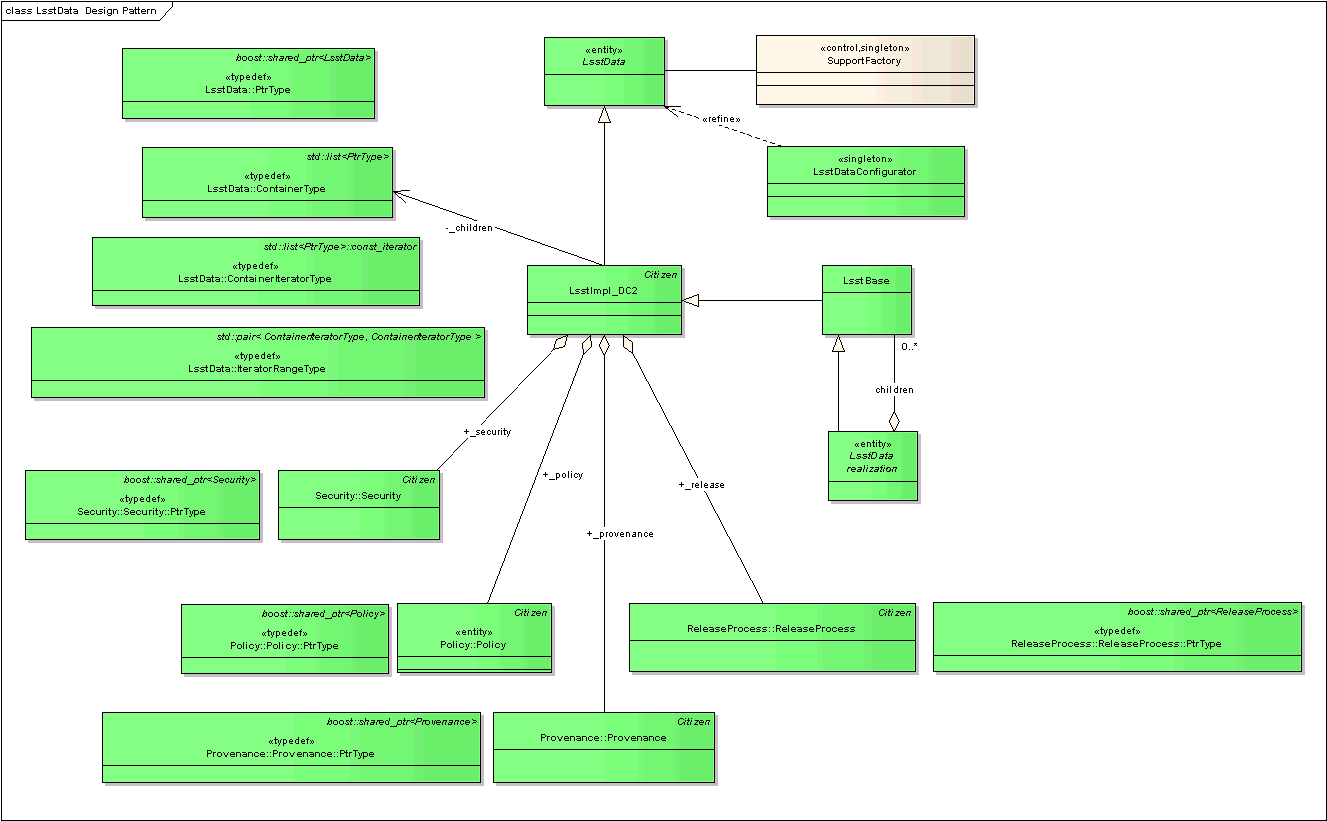
\includegraphics[width=\textwidth]{figures/LsstDataDesign.png}
\caption{\code{SupportFactory}/\code{LsstData}/\code{LsstBase} Design Pattern}
\label{lsstdata-design}
\end{figure}

Ironically, the only DC2 class for which \code{SupportFactory} was generally
used was \code{DataProperty}, somewhat contradicting the goal of having the
latter be a lightweight metadata object.  Heavier-weight classes such as
\code{Image}, \code{WCS}, or \code{Exposure} did not have their instances created using the
\code{SupportFactory} in DC2, even though they did derive from \code{LsstBase}.

In DC3, \code{SupportFactory} will not be used to create \code{DataProperty}
instances.  Its use with other classes may be introduced or mandated,
particularly as we develop functionality for its associated classes
like \code{Provenance} or \code{ReleaseProcess}.

\subsubsection{Policy Class}
\label{Policy}

\paragraph{Description and Usage}

\code{Policy} is a general-purpose class storing hierarchical key/value pairs.
It is intended for read-only data used to configure application
algorithms and pipeline components.  It was initially designed to
support up to three text-based file formats to allow both hand-editing
and machine authoring of configurations: JSON, XML, and an LSST-specific
format called the Policy Authoring Format (PAF).  In the end, JSON
authoring proved to be less popular than PAF, and it requires a
third-party package, so it will be dropped in DC3.  XML support was not
implemented in DC2, but it may become valuable as more complex uses of
\code{Policy}s are developed.

While \code{Policy}s are generally immutable, they do contain a full set of
creation and modification methods.  These are useful for testing, but
there were rare occasions in DC2 where they were used to modify read-in
\code{Policy}s (e.g. substituting for variables in patterns).  These
non-standard uses will be eliminated in the future.

Some additional \code{Policy} capabilities were not fully used in DC2.  The
ability to validate \code{Policy}s based on a dictionary of keys, types, and
values was implemented and many dictionaries were written, but
validation was not required in the final pipelines.  (Compare the
Definition and Dictionary design for the \code{DataProperty} class in
\Sec{DataProperty} above.)  The ability to include \code{Policy} files within
other \code{Policy} files also went unused.


\paragraph{Issues and Lessons Learned}

The underlying model and key/value pair implementation should be shared
with the \code{DataProperty} class, which is otherwise very similar.
\code{Policy} is
a heavier-weight class, as it also incorporates dictionaries and other
features, but the basic key/value operations should be consistent with
\code{DataProperty}.  At the same time, the supported types should be made
consistent, including support for \code{int64\_t} and \code{float}.  All
value types should be accessible from Python, with explicit construction
functions if required.

A request was made to be able to load default \code{Policies} for a pipeline
from a particular directory, overriding values in those \code{Policies} with
new ones from a different \code{Policy} file.

Another request was made to be able to use values set at a higher
level in the \code{Policy} hierarchy as the values of keys at a lower level.
This capability was designed but not implemented in DC2.

Finally, there was a request to be able to parameterize \code{Policy} values
using rules that could test conditions, presumably involving other
values or perhaps even pipeline context information.  The implications
for provenance will need to be explored.

\subsubsection{Persistence Class}
\label{persistence}

\paragraph{Description}

The persistence framework is a set of classes designed to support moving
data to and from persistent storage.  (For simplicity, we will often
refer to persistence instead of both persistence and retrieval.)  This
framework is intended to allow run-time configuration of the destination
of the persistence operation by means of \code{Policy}, to have minimal impact
on the design and implementation of the application class being
persisted, and to support high-performance implementations of
persistence in view of the large amounts of data that the LSST pipelines
will need to create and retrieve.

Persistence is mediated through a \code{Persistence} object that controls the
operation.  \code{Storage} objects provide the interface to the underlying
storage mechanism, while \code{Formatters} control the transformation from
the internal, in-memory format to the external storage format.  The use
of these classes is shown in \Fig{persistence-use}; each class is
described in more detail below.

\begin{figure}[htbp]
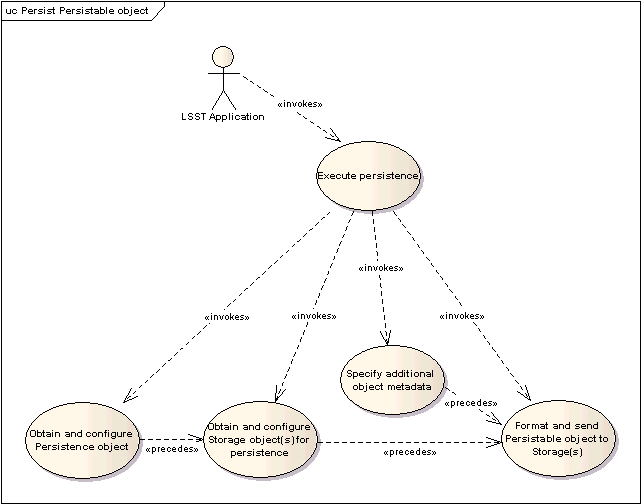
\includegraphics[width=\textwidth]{figures/PersistObject.png}
\caption{Use case for persisting an object}
\label{persistence-use}
\end{figure}

Later during DC2 development, generic input and output pipeline stages
were added to the C++ class framework in order to insulate application
stages from the details of how the data they operate on is retrieved or
persisted.  This allows the application stages to be reusable in more
contexts.

\paragraph{Major Classes}

\Fig{persistence-design} illustrates the design of the major classes in
the persistence framework.

\begin{figure}[htbp]
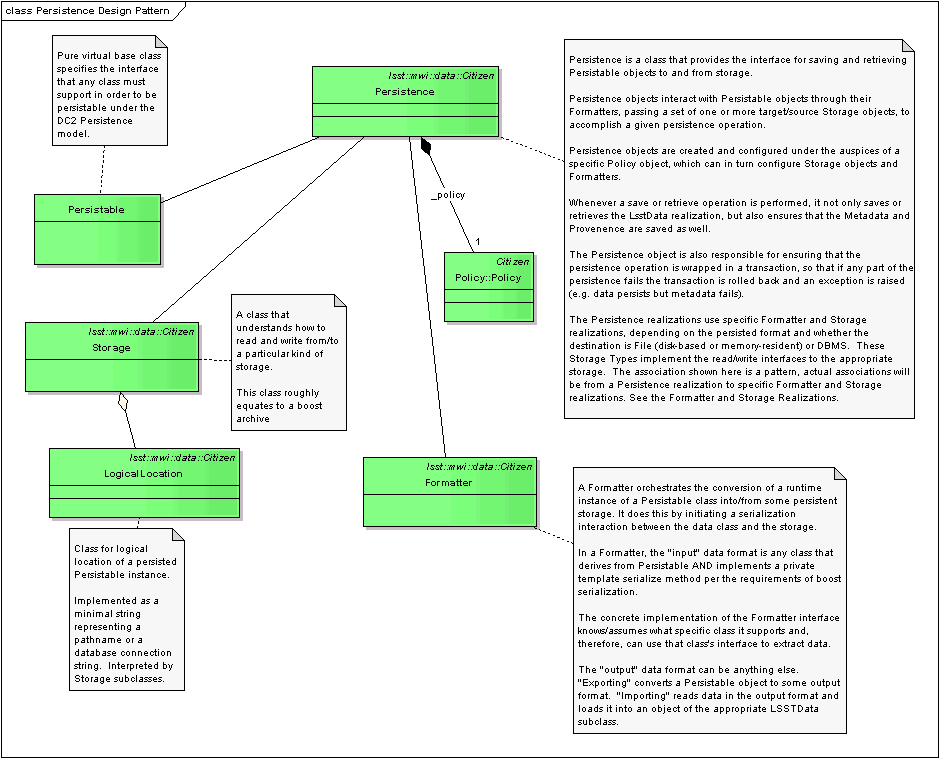
\includegraphics[width=\textwidth]{figures/PersistenceDesign.png}
\caption{Persistence design pattern}
\label{persistence-design}
\end{figure}

\subparagraph{LogicalLocation}
This class encapsulates a URL-like string that provides location
information.

\subparagraph{Storage}
This abstract base class is subclassed for each supported type of
persistent storage (see next section).  Each subclass manages all
interactions with its type of storage and provides methods used by the
\code{Formatter} classes below.  It can accept a \code{Policy} for configuration and
control.

\subparagraph{Formatter}
This abstract base class is subclassed for each persistable application
class.  Each subclass translates the private member variables of its
application class into the appropriate form for persistent storage (or
vice versa).  The subclass must contain code for each type of \code{Storage}
that may be used with the application class.  A \code{DataProperty} of pipeline
information (known as AdditionalData) is passed to the subclass to allow
selection of particular database rows or tables.  The subclass can
accept a \code{Policy} for configuration and control.

\subparagraph{Persistable}
Each persistable application class must inherit from this base class.
It provides the connection with the appropriate \code{Formatter} subclass and
also provides a method used to enable Boost serialization.

\subparagraph{Persistence}
This class manages persistence and retrieval operations.  It provides
access to the factory for \code{Storage} subclasses and selects \code{Formatter}
subclasses based on the type of \code{Persistable}.  It is intended to manage
high-level transactions to ensure the persistence operation completes or
is rolled back, although this functionality was not implemented for DC2.
It, too, can accept a \code{Policy} for configuration and control.

\paragraph{Storage Classes}
\label{Storages}

\subparagraph{DbStorage, DbTsvStorage}
These \code{Storage} subclasses manage the persistence of data to database
tables.  \code{DbTsvStorage} optimizes the persistence of large quantities of
data by writing a temporary tab-separated-value file that is then
bulk-loaded into the database.  These \code{Storages} fully isolate the rest of
the LSST software from the details of database interaction,
encapsulating connections, sessions, table management, value binding,
SQL query creation, prepared statement management, and cursor
operations.  In DC2, they were implemented on top of the CORAL
relational database portability layer from CERN, so they could be
switched from an underlying MySQL database to an Oracle database at
will.  This functionality was found to be unneeded in the short term,
and its cost in terms of the additional package that had to be supported
was relatively high, so in DC3 we will investigate reimplementing these
subclasses directly in terms of the MySQL API.

\subparagraph{FitsStorage}
This simple \code{Storage} manages the pathname needed to persist data to FITS
files in a shared filesystem.

\subparagraph{BoostStorage}
This \code{Storage} manages the persistence of data to text archive files using
the Boost serialization framework.  (Note that some data persisted to
these files may be in binary form for efficiency, despite the
description as ``text archives''.) This \code{Storage} was not used except for
testing.  It will eventually be used for checkpointing the state of
pipelines or stages.

\subparagraph{XmlStorage}
This \code{Storage} is intended to manage the persistence of data to XML files.
This \code{Storage} was not used in DC2.  Its current implementation is in
terms of Boost serialization, which results in a particular form for the
XML file.  If this \code{Storage} is to be used in the future, it may require a
rewrite to handle more general XML structures.

\paragraph{Formatters}

\subparagraph{\code{DataProperty}}
\code{DataProperty} persistence to database storage is used to maintain DC2
provenance information.

\subparagraph{Application framework classes}

While \code{Formatter} subclasses were written for \code{Image},
\code{Mask}, and other application framework classes, the primary one
used in DC2 was \code{Exposure}.  Input and output of \code{Exposure}s
from and to FITS files was supported.  In addition, persistence of
\code{Exposure} metadata, including the WCS, to a database was also
supported.

\subparagraph{Association Pipeline inputs and results}
The vectors of difference image sources (\code{DIASource}s) and moving object
predictions (\code{MopsPred}s) generated by the image processing pipeline and
nightly moving object pipeline, respectively, had \code{Formatter} subclasses
to specify their persistence to database tables (\code{DbTsvStorage}).  The
results of the association pipeline, including vectors of match pairs and
identifier pairs, were also persisted to database tables using \code{Formatter}
subclasses.

\subparagraph{Policy}
\code{Policy} did not use the persistence framework for its text-file retrieval
operations.  Since persistence is configurable by \code{Policy}, doing so would
create a circular dependency.

\paragraph{I/O Stage Classes}

Two pipeline stage classes were added to the distributed processing framework
to support generic input and output of data.  These stages were used in
DC2 to manage all persistence and retrieval of data, with the sole
exception of lookups in the database, for example to obtain filter name
to identifier mappings or moving object orbit parameters.

A sample \code{InputStage} policy looks like this:
\begin{verbatim}
AdditionalData: "exposureId=triggerVisitEvent.exposureId"
InputItems: {
    ScienceExposure: {
        Type: "ExposureF"
        PythonType: "lsst.fw.Core.fwLib.ExposureF"
        StoragePolicy: {
            Storage: "FitsStorage"
            Location: "/lsst/DC2root/%{runId}/ipd/input/%{exposureId}/
                       %{ccdId}/%{exposureId}p_%{ccdId}"
        }
    }
}
\end{verbatim}

The AdditionalData specification allows values from events or
other items on the input clipboard to be made available to the
persistence framework through a \code{DataProperty}.

The InputItems specification gives the item or items to be
retrieved, in this case a ScienceExposure.  Its type information is
provided and the type of storage and location from which to retrieve it
is specified.  The location pathname has substitutions indicated using
``\%\{\}".  Some of these substituted values (e.g. \code{runId}
and \code{ccdId}) are determined by the \code{InputStage} itself based on the
pipeline context; others (e.g. \code{exposureId}) are copied from
clipboard items.  This flexible templating facility allowed any desired
filesystem layout to be easily supported.

A sample \code{OutputStage} policy looks like this:
\begin{verbatim}
AdditionalData: "exposureId=triggerVisitEvent.exposureId"
OutputItems: {
    ScienceExposure: {
        Required: true
        StoragePolicy: {
            Storage: "FitsStorage"
            Location: "/lsst/DC2root/%{runId}/ipd/output/%{exposureId}/
                       %{ccdId}/%{exposureId}p_%{ccdId}"
        }
        StoragePolicy: {
            Storage: "DbStorage"
            Location: "mysql://lsst10.ncsa.uiuc.edu:3306/%{runId}"
        }
    }
}

Persistence: {
    Formatter: {
        ExposureF: {
            ScienceExposure: {
                TableName: "Raw_CCD_Exposure"
            }
        }
    }
}
\end{verbatim}

Here the Required specification is used to indicate that
persistence is mandatory and that the ScienceExposure must be present on
the clipboard.

Two StoragePolicy specifications are used for the single
ScienceExposure; it is persisted first to \code{FitsStorage} and then its
metadata (including the pathname used for the FITS file) is persisted to
\code{DbStorage}.

Finally, the \code{Formatter} subclass for the \code{ExposureF}
application framework class (an instantiation of the general
\code{Exposure} template) is configured to place this ScienceExposure's
metadata into the \code{Raw\_CCD\_Exposure} table in the database.

\paragraph{Performance}

The persistence framework achieved its goal of enabling flexible input
and output of application objects.  Over the course of DC2, the layout
of the input and output files changed several times, but modifications
were limited to the \code{Policy} configurations of the appropriate
\code{InputStage}s or \code{OutputStage}s.  \code{Exposure} persistence
with metadata in the database and pixels in FITS files was demonstrated.
Inter-pipeline communication via the database for difference image
sources and moving object predictions was also demonstrated.

I/O speed was not a limiting bottleneck in the DC2 pipelines, although
this type of performance will need to be monitored carefully in the
future.  Representative times for I/O operations are given in
\Table{tPersist}.

\begin{table}[htb]
\begin{center}
\caption{Timings of I/O operations using the persistence framework}
\label{tPersist}
\vspace{\baselineskip}
\begin{tabular}{| p{0.75\textwidth} | r |}
\hline
Read one slice's 10.3 MB \code{Exposure} and 10.3 MB template
\code{Exposure} from FITS files on NFS filesystem & 9.0 sec \\ \hline
Write one slice's 10.3 MB \code{Exposure} to FITS file on NFS filesystem
and metadata to database & 6.5 sec \\ \hline
Write one slice's 10.3 MB difference \code{Exposure} to FITS file
on NFS filesystem & 6.4 sec \\ \hline
Write one slice's \code{DIASource}s to database \newline
(average number of \code{DIASource}s = 36) & 0.05 sec \\ \hline
Read all \code{DIASource}s from database \newline
(average number of \code{DIASource}s = 1321) & 0.16 sec \\ \hline
Write \code{DIASource} matches to database \newline
(average number of match pairs = 1082) & 0.03 sec \\ \hline
Write new \code{Object} identifier pairs to database \newline
(average number of pairs = 537) & 0.02 sec \\
\hline
\end{tabular}
\end{center}
\end{table}

Note that DC2 was limited to a single-host NFS filesystem for image
storage.  As a result, while the per-slice I/O bandwidths achieved were
only on the order of 1.6--2.3 MB/sec, the overall I/O bandwidth to the
shared filesystem was a much more reasonable 57--83 MB/sec, especially
given the contention involved with 36 simultaneous I/O operations.

In the future, we expect to use an image store that has much larger
aggregate bandwidth and lower contention.  This might be implemented,
for example, by providing SAN connections to each compute node or by
using a Lustre parallel filesystem.  The result would be significantly
decreased image read and write times and increased scalability.

\paragraph{Issues and Lessons Learned}

A common persistence use case occurring during testing and manual
debugging is to persist an application object to a single type of
storage.  Performing this operation currently requires several steps in
Python.  A convenience function to simplify this use case into a single
step will be provided.

Information used to specify the location of persisted objects is
provided in various places, including the AdditionalData
\code{DataProperty}, the Location in the StoragePolicy specification of
the \code{InputStage} or \code{OutputStage}, and in some cases items in
the \code{Formatter} \code{Policy}.  These should be merged
into a single \code{DataProperty}, perhaps as part of the
\code{LogicalLocation}.

The facility for substituting values into the location strings is
valuable, powerful, and flexible, but it adds yet another syntax to
learn.  The standard Python syntax and formatting mechanisms will be
used to simplify usage.
